\section{Motivation}\label{sec:motivation}

\subsection{Low-Latency Applications}

The main motivation for shifting computation from cloud to edge infrastructure is to mitigate network latency. In specific, real-time applications are the main candidates for benefiting of services deployed at nearby edge infrastructure. Among these, some have a higher degree of criticallity with respect to latency and readiness of services (e.g., delay can have severe consequences to the users and/or the environment), whereas others can greatly benefit from lower latencies (e.g., by improving the user experience).

As an example of a critical application, connected vehicles~\cite{} are expected to be the computing device of the next decade. They are expected to generate XX petabytes of data by XXXX year~\cite{connectedCars} \textcolor{blue}{how much, cite survey}
. In addition to local data analysis, more complex analysis shall be delegated to remote servers, which must respond quickly if the result involves critical information, e.g., the notification of an accident in the current path of the vehicle. With edge computing, computational resources located at mobile base stations or even composing the traffic infrastructure (e.g., highways) could provide low-latency services for connected vehicles passing by their coverage area.

Moreover, Augmented Reality (AR) is a type of application that would benefit from the low-latency of edge services~\cite{hu2015mobile,GarrigaMendonca2017}. These applications enrich the interaction of users with the physical
world by augmenting their vision of the reality with relevant information (e.g., historical information about buildings and monuments), modifying it (e.g., by translating captured text in a different language), or by adding virtual elements that can mimic interactions with the real world (e.g., virtual objects or creatures
from a fantasy game), or helping users fulfill physical tasks (e.g., by highlighting a free parking spot).

AR applications commonly depend on two key computational tasks: 1) extracting features from physical elements in the captured scene; and 2) matching these features against a feature database to obtain the corresponding information to be added to the scene. 

With the advent of mobile computing, AR applications can be deployed to companion devices like smartphones, tablets, and special purpose glasses. In many cases, these applications must process large volumes of data. Plus, this data can be volatile, which further limits the feasibility of storing it locally. Instead, data must be acquired from remote services. In order to augment the reality captured live from devices camera, the AR application needs to perform its tasks in a timely fashion, which poses a strong restriction on the latency requirement for remote services consumed. As such, a cloud-based solution tends to fail to meet this requirement~\cite{ServerlessEdgeESOCC17}. 

%Additionally, image processing may over stress devices resources. This problem could be mitigated  
%architectural decision of where these tasks should be computed.

%AR applications that capture a live representation of the physical world, this reality must be augmented at real-time, meaning data must be retrieved in a timely fashion. Due to network latency, a cloud-based solution tends to fail. Accordingly, feature extraction task should be deployed near to client devices, e.g.., to edge servers. 

\begin{figure}[tbp]
	\centering
	\subfloat[first caption.\label{fig:cloud-to-edge}]{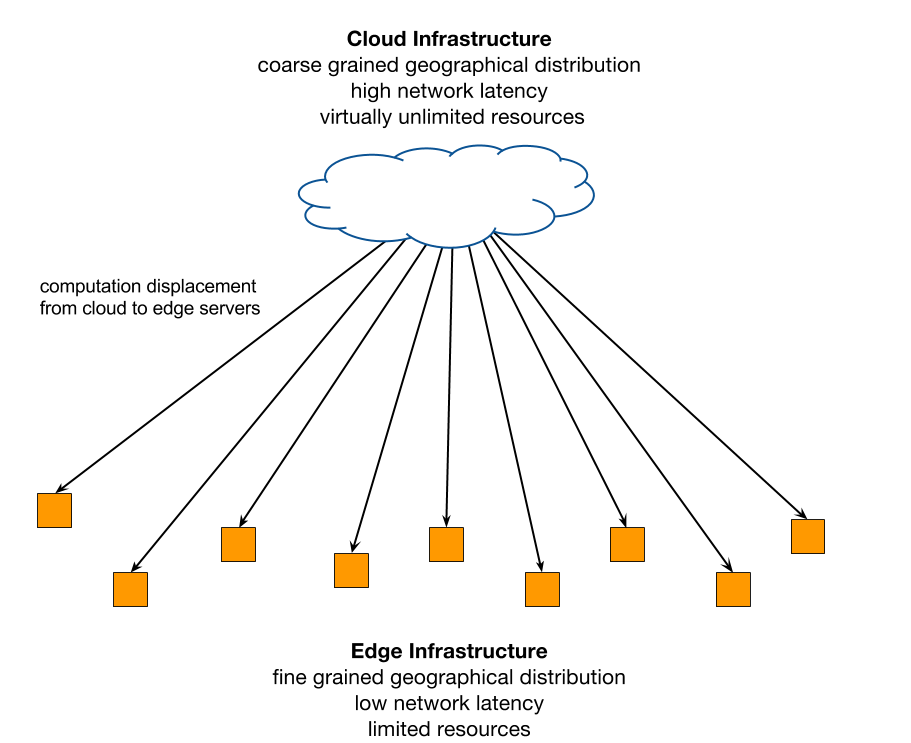
\includegraphics[width=0.49\textwidth]{figs/cloud-to-edge.png}}\hfill
	~
	\subfloat[second caption.\label{fig:mobile-to-edge}] {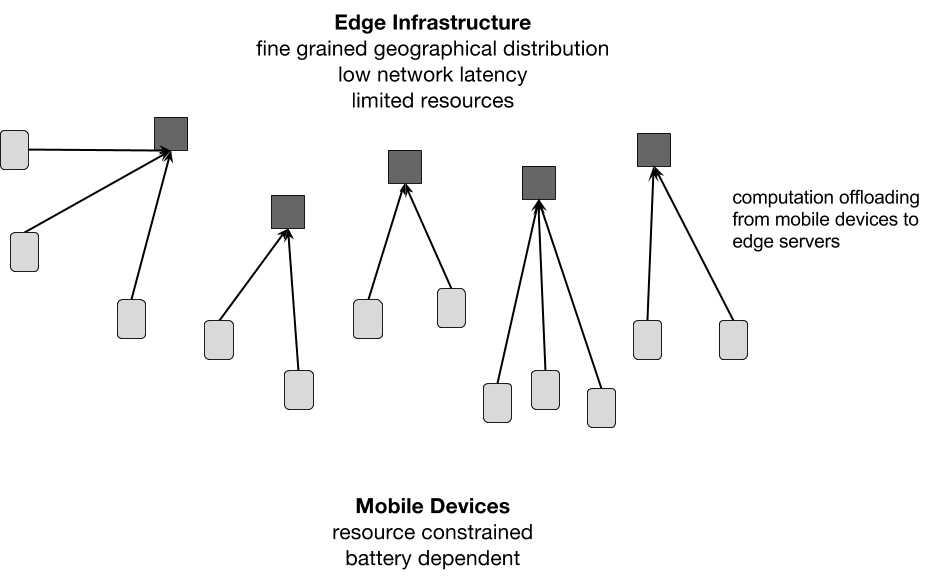
\includegraphics[width=0.49\textwidth]{figs/mobile-to-edge.png}}\hfill
	\caption{General caption.} \label{fig:1}
\end{figure}

\subsection{Mobile Computation Offloading}

In addition to the problem of network latency, mobile devices exhibit limitations that may further motivate the use of edge computing. 

For instance, some mobile applications rely on heavyweight tasks that can overstress the platform and limit the concurrent execution of other applications. Moreover, battery is a valuable resource that may be significantly affected by the kind of computational task performed by mobile devices. 

In the paradigm of Mobile Cloud Computing (MCC)~\cite{Khan:14}, this problem has been addressed with the offloading of mobile computation to cloud servers. This approach, however, is limited by network latency. In contrast, edge computing could be an alternative to allow heavyweight or complex computation with low-latency requirements to be offloaded from resource constrained devices to nearby servers.

%The paradigm of edge computing can be explored to mitigate the problems related to the resource limitations of mobile devices. For this, heavyweight computation from mobile applications could be offloaded to nearby edge servers. 

As an example, the previously mentioned feature extraction task from AR applications is a type of heavyweight computation based on image processing. Instead of performing it locally (as proposed in~\cite{Huang2012}), mobile devices could also offload this task to nearby edge servers. 

\subsection{Computational Continuum}

TODO: add the image representing the computational continuum

Together, the computational resources from mobile, edge, and cloud computing have the potential of forming a \textit{\textbf{computational continuum}} on which new and disruptive types of applications can rely. 

To illustrate such scenario, we put together the two application examples previously described as part of a continuum that starts in the user's office and finishes in his home. 

In the office, let's assume the existence of a local edge server, which will be called from now on \textit{local-edge}. This server is owned by the company to allow employees to extend the computational capabilities of their tablet devices. Our user, e.g., makes use of an augmented reality application to TODO: describe here how an employee would use AR at work or change it to a home scenario.

After work, the user leaves his office and enters his connected vehicle. During its way home, this autonomous vehicle will make use of nearby edge computing servers deployed at cellular base stations and owned by telecoms, which will be called from now on \textit{mobile-edge}. In specific, the connected vehicle gets updates about the best plan to reach its destination, considering the multitude of other users been driven home during the hush hour. For instance, within milliseconds, the vehicle is suggested to make a turn just in time to avoid the traffic formed by an accident two blocks ahead. 

Already at home, the user's smartphone gets in reach of communication with the local-edge server owned by him. The user finds out about a new mobile game application that makes use of augmented reality. Upon installation, the local-edge server becomes aware of a new edge-compliant application and proceeds with the acquisition and deployment of the game components and assets that will be exposed as a service. After this, the game application, which was already running locally, becomes aware of the edge service and starts consuming it with the purpose of offloading computation and preserving the smartphone resources. Not only the game performance improves, but also the battery consumption is reduced.  

In the scenario above, different types of edge infrastructure have been employed by user's devices. In specific, our idea of a computation continuum refers to the pervasiveness of computational resources and to the seamlessly transition of computation among mobile, edge, and cloud resources. Needless to say, for all the applications cited above, cloud infrastructure is  fundamental, as different services for which network latency is not disruptive are still in the cloud (e.g., persistence and large part of the business logic).